\setcounter{figure}{0}

\section{2nd April 2023: Fall of Babylon}
\subsection*{Text: Revelation 17:1-18:24}
  \begin{quote}
    [1] Then one of the seven angels who had the seven bowls came and said to me, “Come, I will show you the judgment of the great prostitute who is seated on many waters, [2] with whom the kings of the earth have committed sexual immorality, and with the wine of whose sexual immorality the dwellers on earth have become drunk.” [3] And he carried me away in the Spirit into a wilderness, and I saw a woman sitting on a scarlet beast that was full of blasphemous names, and it had seven heads and ten horns. [4] The woman was arrayed in purple and scarlet, and adorned with gold and jewels and pearls, holding in her hand a golden cup full of abominations and the impurities of her sexual immorality. [5] And on her forehead was written a name of mystery: “Babylon the great, mother of prostitutes and of earth’s abominations.” [6] And I saw the woman, drunk with the blood of the saints, the blood of the martyrs of Jesus.

    When I saw her, I marveled greatly. [7] But the angel said to me, “Why do you marvel? I will tell you the mystery of the woman, and of the beast with seven heads and ten horns that carries her. [8] The beast that you saw was, and is not, and is about to rise from the bottomless pit and go to destruction. And the dwellers on earth whose names have not been written in the book of life from the foundation of the world will marvel to see the beast, because it was and is not and is to come. [9] This calls for a mind with wisdom: the seven heads are seven mountains on which the woman is seated; [10] they are also seven kings, five of whom have fallen, one is, the other has not yet come, and when he does come he must remain only a little while. [11] As for the beast that was and is not, it is an eighth but it belongs to the seven, and it goes to destruction. [12] And the ten horns that you saw are ten kings who have not yet received royal power, but they are to receive authority as kings for one hour, together with the beast. [13] These are of one mind, and they hand over their power and authority to the beast. [14] They will make war on the Lamb, and the Lamb will conquer them, for he is Lord of lords and King of kings, and those with him are called and chosen and faithful.”

    [15] And the angel said to me, “The waters that you saw, where the prostitute is seated, are peoples and multitudes and nations and languages. [16] And the ten horns that you saw, they and the beast will hate the prostitute. They will make her desolate and naked, and devour her flesh and burn her up with fire, [17] for God has put it into their hearts to carry out his purpose by being of one mind and handing over their royal power to the beast, until the words of God are fulfilled. [18] And the woman that you saw is the great city that has dominion over the kings of the earth.”

    [1] After this I saw another angel coming down from heaven, having great authority, and the earth was made bright with his glory. [2] And he called out with a mighty voice,

    “Fallen, fallen is Babylon the great!
        She has become a dwelling place for demons,
    a haunt for every unclean spirit,
        a haunt for every unclean bird,
        a haunt for every unclean and detestable beast.
    [3] For all nations have drunk
        the wine of the passion of her sexual immorality,
    and the kings of the earth have committed immorality with her,
        and the merchants of the earth have grown rich from the power of her luxurious living.”


    [4] Then I heard another voice from heaven saying,

    “Come out of her, my people,
        lest you take part in her sins,
    lest you share in her plagues;
    [5] for her sins are heaped high as heaven,
        and God has remembered her iniquities.
    [6] Pay her back as she herself has paid back others,
        and repay her double for her deeds;
        mix a double portion for her in the cup she mixed.
    [7] As she glorified herself and lived in luxury,
        so give her a like measure of torment and mourning,
    since in her heart she says,
        ‘I sit as a queen,
    I am no widow,
        and mourning I shall never see.’
    [8] For this reason her plagues will come in a single day,
        death and mourning and famine,
    and she will be burned up with fire;
        for mighty is the Lord God who has judged her.”


    [9] And the kings of the earth, who committed sexual immorality and lived in luxury with her, will weep and wail over her when they see the smoke of her burning. [10] They will stand far off, in fear of her torment, and say,

    “Alas! Alas! You great city,
        you mighty city, Babylon!
    For in a single hour your judgment has come.”


    [11] And the merchants of the earth weep and mourn for her, since no one buys their cargo anymore, [12] cargo of gold, silver, jewels, pearls, fine linen, purple cloth, silk, scarlet cloth, all kinds of scented wood, all kinds of articles of ivory, all kinds of articles of costly wood, bronze, iron and marble, [13] cinnamon, spice, incense, myrrh, frankincense, wine, oil, fine flour, wheat, cattle and sheep, horses and chariots, and slaves, that is, human souls.

    [14] “The fruit for which your soul longed
        has gone from you,
    and all your delicacies and your splendors
        are lost to you,
        never to be found again!”


    [15] The merchants of these wares, who gained wealth from her, will stand far off, in fear of her torment, weeping and mourning aloud,

    [16] “Alas, alas, for the great city
        that was clothed in fine linen,
            in purple and scarlet,
        adorned with gold,
            with jewels, and with pearls!
    [17] For in a single hour all this wealth has been laid waste.”


    And all shipmasters and seafaring men, sailors and all whose trade is on the sea, stood far off [18] and cried out as they saw the smoke of her burning,

    “What city was like the great city?”


    [19] And they threw dust on their heads as they wept and mourned, crying out,

    “Alas, alas, for the great city
        where all who had ships at sea
        grew rich by her wealth!
    For in a single hour she has been laid waste.
    [20] Rejoice over her, O heaven,
        and you saints and apostles and prophets,
    for God has given judgment for you against her!”


    [21] Then a mighty angel took up a stone like a great millstone and threw it into the sea, saying,

    “So will Babylon the great city be thrown down with violence,
        and will be found no more;
    [22] and the sound of harpists and musicians, of flute players and trumpeters,
        will be heard in you no more,
    and a craftsman of any craft
        will be found in you no more,
    and the sound of the mill
        will be heard in you no more,
    [23] and the light of a lamp
        will shine in you no more,
    and the voice of bridegroom and bride
        will be heard in you no more,
    for your merchants were the great ones of the earth,
        and all nations were deceived by your sorcery.
    [24] And in her was found the blood of prophets and of saints,
        and of all who have been slain on earth.”
  \end{quote}

\subsection*{Notes}
\begin{itemize}
  \item{Here, we have an elaboration of the seventh bowl, which contains a
  judgment of Babylon.  It is as if God drew back a curtain to reveal what
  Babylon really was; the city looked very splendid from the outside, but the
  city was actually very wicked.}
  \item{Three points for today:
  \begin{itemize}
    \item{Disposition of the city}
    \item{Demise of the city}
    \item{Decision of God's people}
  \end{itemize}}
  \item{On Rev 17:5, was written on the forehead of the woman who personifies
  the city: ``And on her forehead was written a name of mystery: Babylon the
  great, mother of prostitutes and of earth's abominations''.  The name here
  reveals the true character and disposition of Babylon.  The city, from an
  external POV, was really great, spanning many mountains.  But internally,
  the city was full of rot.  The epithet ``mother of prostitutes'' means that
  Babylon is the source of all prostitutes.  In the city for example, there
  is a lot of decadence and a lot of debauchery.  But the metaphor of a
  prostitute means that Babylon is guilty of more than just sexual
  immorality.  The metaphor of a prostitute means that Babylon was also
  guilty of enticing people to sexual immorality.  And as we all know, sexual
  immorality in the Bible (especially the OT) is linked to idolatry; idolatry
  is described with the metaphor of sexual immorality (c.f Hosea).  \\ The
  outward appearance of the city was also described in very alluring terms,
  unlike the beast who had a fearsome appearance.  This describes how the
  city could be very tempting to other people.  The woman personifying the
  city is also described as ``drunk with the blood of God's people''.  This
  city was built on the suffering of the saints.  Babylon here, as described
  by John, is not exactly the Babylon of the OT.  Babylon here is the name
  for all earthly world powers/systems who set themselves against God.  It is
  a reminder to God's people that in every age, there will be a Babylon that
  is bent on opposing God and instigating ungodliness and enticing God's
  people to idolatry.  }
  \item{As God's people, we must be wary of the seduction of power, wealth
  and pleasure (which Babylon exemplifies) lest we end up being unfaithful to
  God.  To guard against being enticed by Babylon, there are these things we
  can do:
  \begin{itemize}
    \item{We can cultivate contentment.  We need to crucify this
    consumeristic spirit that is so rife in the modern world.  To do so, we
    can be more intentional with thanksgiving.}
    \item{We can count the `cost'.  When we are tempted to fall into the ways
    of the world (which are very enticing), we should count the `cost' of
    doing so.  How would our actions affect our soul, and the people around
    us?  How would it affect our Christian witness?  Etc.  }
  \end{itemize}}
  \item{Now that we have described the disposition of the city, we shall
  describe the demise of the city.  One very interesting thing to see here is
  that Babylon will be betrayed by the beast which once supported her.  We
  see how in God's judgment, God's enemies will be treacherous to each other.
  This tells us that when we take evil as an ally, the evil will eventually
  betray us and let us down (compare this with the faithfulness of God).
  Also, we see that when the city is judged by God, the ``merchants of the
  earth weep and mourn for her, since no one buys their cargo anymore''.  We
  see that through God's judgment, the idols of the world are exposed.  Also,
  we see that when Babylonn was judged, there was much silence in the city.
  No more harpists etc.  On the other hand, there was much rejoicing in
  heaven.  Through God's judgement, God's people are vindicated.  Note that
  the rejoicing of God's people here is not them laughing at their enemies.
  It is them feeling vindicated that the faithful life that they led will
  finally vindicate them, and it is them rejoicing that justice has been
  meted out. }
  \item{For us then, given the certainty of God's judgement, God's people are
  not to be overcome by evil but overcome evil with good by being faithful to
  God.  We must show the world that there is a better way to live.}
  \item{Now, what is the decision that God's people must make?  It is to
  ``come out of her, my people, lest you take part in her sins, lest you
  share in her plagues...''.  As God's people, we must consecrating
  ourselves.  We must remind outselves first and foremost that we belong to
  Christ, and that we have been purchased by the blood of the Lamb.  One easy
  way to do this is to gather as God's people for worship on the Lord's day!
  The harder thing to do is to live holy lives, to deny ourselves (in
  contrast to the world's mantra to love yourself).  That is how we can
  consecrate ourselves.}
  \item{Another thing we can do is to call out wrongdoing.  We are to call
  out injustice when we see it.  We are badgered by the world not only to
  tolerate sin, but sometimes to celebrate sin.  We must resist that and be
  firm in our convictions and also be firm in speaking out our convictions.
  This command to ``come out'' is not a legalistic command, it is more of an
  invitation to a life of freedom and fullness in Christ.  Living like the
  world, living in Babylon, is bondage and burdensome.  Living in Babylon
  will never satisfy, and it will drive us to chase things that are vanity.
  The invitation to ``come out of Babylon'' would then be an invitation to
  fullness of life in Christ, through in a practical sense, there will also
  be suffering.  But yet the suffering in this world is to be counted as
  nothing in light of the eternal joy and bliss we will have when Jesus comes
  again.  So let us live with eternity in mind, and come out of Babylon.  }
  \item{\begin{figure}[H]
    \centering
    % 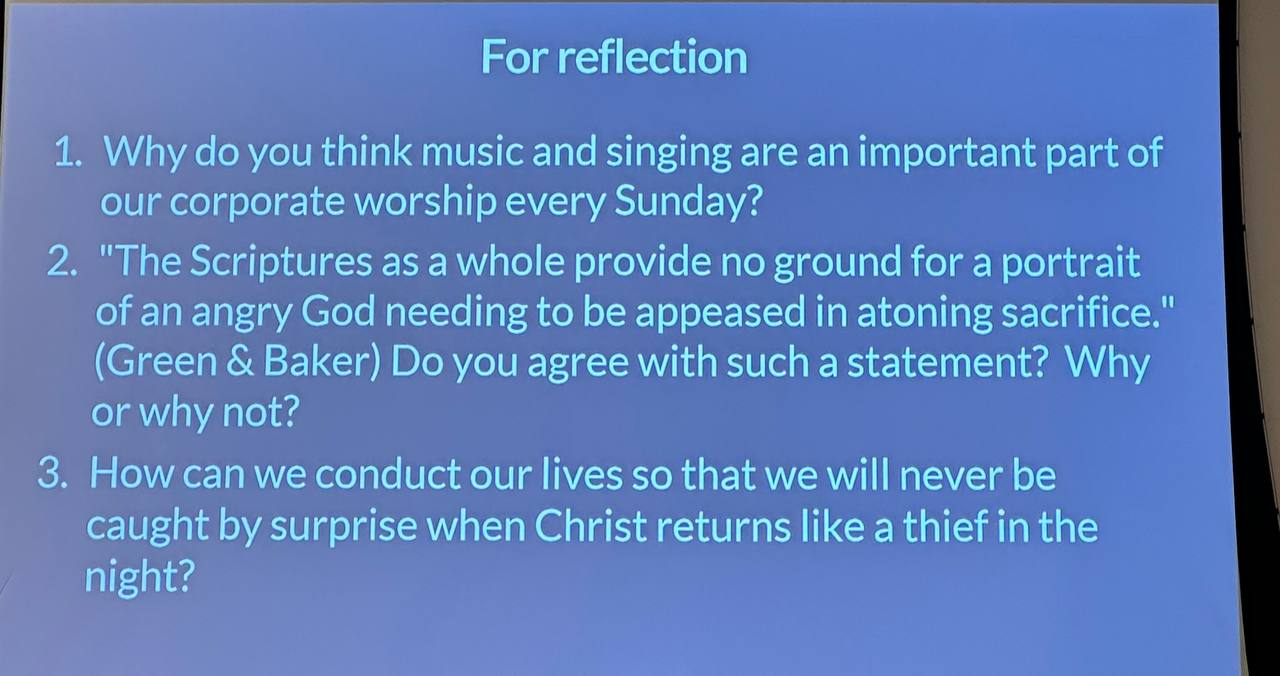
\includegraphics[width=0.8\textwidth, trim={0cm 0cm 0cm 0cm},clip]{Figures/marSermon4Reflections.jpg}
    \includegraphics[width=0.8\textwidth, trim={0cm 0cm 0cm 0cm},clip]{example-image-a}
    \caption[]{Reflection questions for this sermon}
    \label{}
  \end{figure}}
\end{itemize}